\chapter{Foundational Algebra and Analysis}

I want you to restart from scratch - I want to change the way you imagine \textit{Mathematics}. I want you to visualise most of its concepts and appreciate its beauty. \\

Let's start with the most basic question possible - \textit{What is mathematics?} In my opinion, mathematics is the study of abstractions. The first and foremost abstract idea is the \textit{number}. Numbers are the direct consequence of our ability to count. When I mention 3 or 6, you understand the quantity without considering what is being counted; the focus is on the act of counting, making the number itself an abstract entity. Despite it being such an abstract entity, we have been able to  work with it and have developed theories of mathematics around it - from algebra to calculus, from analysis to probability theory and what not. \\

But knowing numbers isn't enough. We have to extend this idea of abstractions before we dive deep into the probability theory. 

\setlength{\headheight}{14.49998pt}
\addtolength{\topmargin}{-2.49998pt}

\section{The Abstraction of Mathematical Ideas}

To explain what I mean by \textit{abstraction} - the word that I have used dozens of times by now, I will present three seemingly unrelated ideas in mathematics and demonstrate how they converge into a single concept when thought abstractly.

\subsection{Idea 1: Matrix Multiplication and Permutation Matrices} 

\vspace{3pt} 
The first example comes from the course on \textit{Linear Algebra}. \textit{Have you ever wondered why you multiply two matrices the way you do?} It seems so bizzare that when you are adding two 3 $\times$ 3 matrices, you are adding elementwise; but when you are multiplying them, then suddenly a weird rule of multiplying rows with columns comes into picture. \textit{Why?} \\

I expect you are fami
liar with the facts that columns of a matrix are \textit{vectors} and $n$ simultaneous linear equations with $n$ variables can be written in the matrix form $AX = B$, where $A$ is the $n \times n$ coefficient matrix, $X$ is the $n \times 1$ matrix of unknowns and $B$ is the $n \times 1$ resultant vector. Geometrically, since each column of the coefficient matrix is a vector in $n$ dimensions, if they are \textit{linearly independent}, we will be able to find a solution i.e. a list of linear combination coefficients $X$ such that a linear combination of those vectors in $A$ gets us the resultant vector $B$. \\

By the nature of the visualization itself in the column picture, if we were to find not just a single linear combination that results in $B$, but two more linear combinations that result in vectors $C$ and $D$ too, the equation becomes 

\begin{center}
$A \cdot \begin{bmatrix} X_1 & X_2 & X_3 \end{bmatrix} = \begin{bmatrix} B & C & D \end{bmatrix}$
\end{center}

If you put the appropriate elements in this matrix, and try to write three linear combinations i.e. three sets of simultaneous linear equations, you will see the reason - why we multiply the matrices the way we do so. From this idea, it should also get clear that the multiplication $A.B$ has a different meaning than $B.A$. This implies, matrix multiplication is not commutative.\\

\textit{But why do we care so much about matrix multiplications?} Because we want to understand the impact on a matrix when it is multiplied by another matrix. \\

Now that we know matrix multiplication is a collection of linear combinations \textit{(this idea is further refined to be called as \textbf{linear transformation})}, we can easily confirm that - if $AB = B$, then $A$ should have a form where diagonal elements are 1 and rest are 0. It's the \textit{identity matrix}. \\

Let's do a reverse-engineering exercise. If

\begin{equation}
    E.
    \begin{bmatrix}
        1 & 2 & 1 \\
        3 & 8 & 1 \\
        0 & 4 & 1
    \end{bmatrix}
    =
    \begin{bmatrix}
        1 & 2 & 1 \\
        0 & 2 & -2 \\
        0 & 4 & 1
    \end{bmatrix}
\end{equation}

then what is $E$? \\

From the first look it is clear that $E$ is very close to the identity matrix as only the second row is different. If we sum three negatives of [1 2 1] and one positive of [3 8 1], we will get [0 2 -2]. Hence, 

$$
E =
\begin{bmatrix}
    1 & 0 & 0 \\
    -3 & 1 & 0 \\
    0 & 0 & 1
\end{bmatrix}
$$

Now what if I have to nullify the effect of multiplication of $E$ shown above on $A$? We should add 3 times the first row to the second row, to compensate for subtracting three times the first row from the second. Notice how the elements of the matrix are acting as row-selectors. 

$$
E^{-1} =
\begin{bmatrix}
    1 & 0 & 0 \\
    3 & 1 & 0 \\
    0 & 0 & 1
\end{bmatrix}
$$

And we can confirm that their effects nullify, because $E.E^{-1} = I$. This gives us the concept of \textit{inverses} in matrices. The matrices that you shall encounter will be very complex, but the core principle behind the matrix multiplication remains the same. 

\subsubsection{Permutation Matrices}

Recall, that the matrix equation $AX = B$ is the set of $n$ equations with $n$ variables. The order in which these equations appear should have no impact on the final solution. This implies, that rows can come in any permutation, the final solution remains unchanged. The matrix $P$ whose effect when multiplied on $A$ is to reorder the rows of $A$ is called the \textit{permutation matrix}. \\

In a $3D$ space, there are 6 permutation matrices, as shown below. \\

\[
\begin{bmatrix}
1 & 0 & 0 \\
0 & 1 & 0 \\
0 & 0 & 1
\end{bmatrix}
\hspace{1em}
\begin{bmatrix}
1 & 0 & 0 \\
0 & 0 & 1 \\
0 & 1 & 0
\end{bmatrix}
\hspace{1em}
\begin{bmatrix}
0 & 1 & 0 \\
1 & 0 & 0 \\
0 & 0 & 1
\end{bmatrix}
\hspace{1em}
\begin{bmatrix}
0 & 1 & 0 \\
0 & 0 & 1 \\
1 & 0 & 0
\end{bmatrix}
\hspace{1em}
\begin{bmatrix}
0 & 0 & 1 \\
1 & 0 & 0 \\
0 & 1 & 0
\end{bmatrix}
\hspace{1em}
\begin{bmatrix}
0 & 0 & 1 \\
0 & 1 & 0 \\
1 & 0 & 0
\end{bmatrix}
\] \\

\textit{\textbf{Note:}} The elements of the above set of permutation matrices are representing some sort of \textit{action}. The effect of the \textit{action} is to reorder the rows of the matrix on which the permutation matrix is operated on. To operate any permutation matrix $P$ on $A$, you have to left-multiply $P$ on $A$. 

\subsection{Idea 2: Symmetries of a Triangle}

Imagine we have a shape of a triangle. The question is - \textit{what kind of operations can I perform on this shape?} Clearly, this is a shape. It's not a number on which we can perform addition or multiplication or any such operation which we would define for a number. The only two actions that are possible to perform on this shape are: \textit{rotation} and \textit{reflection}. You can rotate this triangle by some angle or you can flip it. \\

But, \textit{why are we performing these operations? What's our agenda?} The agenda is we want to learn about the symmetries of triangle. Understanding  symmetries involves exploring different ways a triangle can be transformed while preserving its appearance. We will examine how a triangle can be rotated or flipped to match its original position. \\

Consider the triangle \( ABC \) as shown below.

\begin{center}
    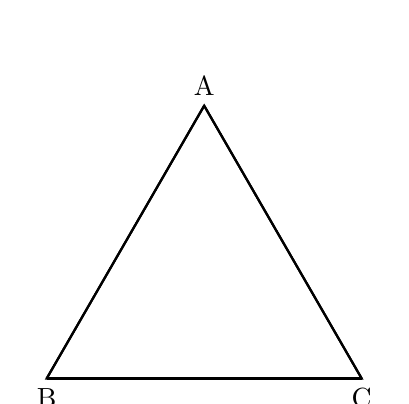
\begin{tikzpicture}
        % Draw the triangle
        \draw[thick] (0,0) -- (4,0) -- (2,3.464) -- cycle;
        
        % Label the vertices
        \node at (0,0) [below] {B};
        \node at (4,0) [below] {C};
        \node at (2,3.464) [above] {A};
        
        % Optionally, draw the sides
        \draw[thick] (0,0) -- (4,0); % AB
        \draw[thick] (4,0) -- (2,3.464); % BC
        \draw[thick] (2,3.464) -- (0,0); % CA
        
        \end{tikzpicture}
\end{center}

\subsubsection{Rotations}

Rotations involve turning the triangle around its center. The triangle can be rotated by angles that are multiples of \( \frac{360^\circ}{3} = 120^\circ \).

\begin{itemize}
    \item \textbf{Rotation by \( 0^\circ \):} This is the identity rotation, where the triangle remains unchanged. This is represented by:
    \[
    \text{Identity: } \text{Triangle} \rightarrow \text{Triangle}
    \]
    
    \item \textbf{Rotation by \( 120^\circ \):} Rotating the triangle by \( 120^\circ \) counterclockwise about its center maps each vertex to the position of the next vertex in a counterclockwise direction. We denote this rotation as \( R_{120^\circ} \). In a triangle with vertices \( A, B, \) and \( C \), the effect is:
    \[
    R_{120^\circ}: A \rightarrow B, \; B \rightarrow C, \; C \rightarrow A
    \]
    
    \item \textbf{Rotation by \( 240^\circ \):} This rotation maps each vertex to the position of the previous vertex in a counterclockwise direction. We denote this rotation as \( R_{240^\circ} \). For vertices \( A, B, \) and \( C \), the effect is:
    \[
    R_{240^\circ}: A \rightarrow C, \; B \rightarrow A, \; C \rightarrow B
    \]
\end{itemize}

\begin{center}
    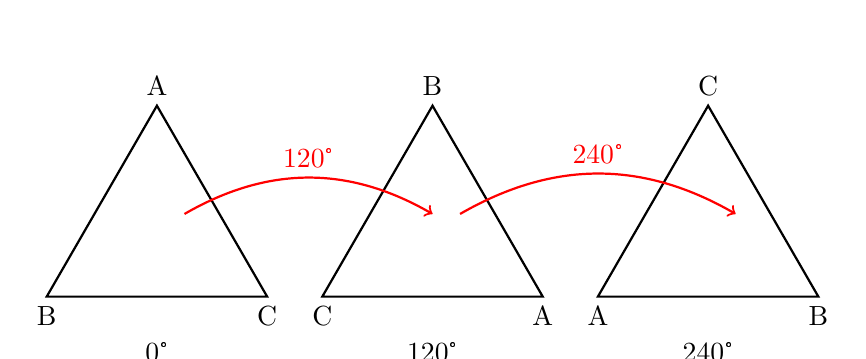
\begin{tikzpicture}[scale=0.7]
        % Original Triangle (0 degrees)
        \begin{scope}[shift={(-5,0)}]
            \draw[thick] (0,0) -- (4,0) -- (2,3.464) -- cycle;
            \node at (0,0) [below] {B};
            \node at (4,0) [below] {C};
            \node at (2,3.464) [above] {A};
            \node at (2,-1) {0°};
        \end{scope}
        
        % Rotated 120 degrees
        \begin{scope}[shift={(0,0)}]
            \draw[thick] (0,0) -- (4,0) -- (2,3.464) -- cycle;
            \node at (0,0) [below] {C};
            \node at (4,0) [below] {A};
            \node at (2,3.464) [above] {B};
            \node at (2,-1) {120°};
        \end{scope}
        
        % Rotated 240 degrees
        \begin{scope}[shift={(5,0)}]
            \draw[thick] (0,0) -- (4,0) -- (2,3.464) -- cycle;
            \node at (0,0) [below] {A};
            \node at (4,0) [below] {B};
            \node at (2,3.464) [above] {C};
            \node at (2,-1) {240°};
        \end{scope}
        
        % Transition arrows between triangles
        \draw[->,thick,red] (-2.5,1.5) to[bend left] node[midway,above] {120°} (2.0,1.5);
        \draw[->,thick,red] (2.5, 1.5) to[bend left] node[midway,above] {240°} (7.5,1.5);
    \end{tikzpicture}
\end{center}

\subsubsection{Reflections}

Reflections involve flipping the triangle over a line of symmetry. A triangle has three lines of symmetry, each passing through a vertex and the midpoint of the opposite side.

\begin{itemize}
    \item \textbf{Reflection over the line through \( A \) and the midpoint of \( BC \):} This reflection maps the triangle to itself by flipping it over the line passing through vertex \( A \) and the midpoint of the side \( BC \). We denote this reflection as \( F_A \):
    \[
    F_A: B \leftrightarrow C, \; A \text{ remains fixed}
    \]
    
    \item \textbf{Reflection over the line through \( B \) and the midpoint of \( AC \):} This reflection maps the triangle to itself by flipping it over the line passing through vertex \( B \) and the midpoint of the side \( AC \). We denote this reflection as \( F_B \):
    \[
    F_B: A \leftrightarrow C, \; B \text{ remains fixed}
    \]
    
    \item \textbf{Reflection over the line through \( C \) and the midpoint of \( AB \):} This reflection maps the triangle to itself by flipping it over the line passing through vertex \( C \) and the midpoint of the side \( AB \). We denote this reflection as \( F_C \):
    \[
    F_C: A \leftrightarrow B, \; C \text{ remains fixed}
    \]
\end{itemize}

\begin{center}
    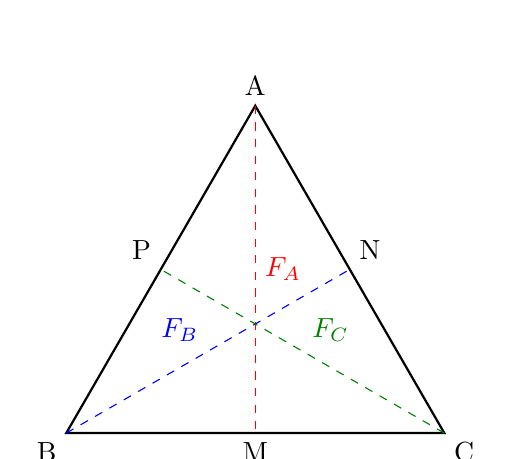
\begin{tikzpicture}[scale=1.2]
        % Define coordinates
        \coordinate (A) at (0,3.464);
        \coordinate (B) at (-2,0);
        \coordinate (C) at (2,0);
        
        % Draw the main triangle
        \draw[thick] (A) -- (B) -- (C) -- cycle;
        
        % Label vertices
        \node[above] at (A) {A};
        \node[below left] at (B) {B};
        \node[below right] at (C) {C};
        
        % Draw and label perpendicular bisectors
        \draw[red, dashed] (A) -- (0,0) node[midway, right] {$F_A$};
        \draw[blue, dashed] (B) -- (1,1.732) node[midway, above left] {$F_B$};
        \draw[green!50!black, dashed] (C) -- (-1,1.732) node[midway, above right] {$F_C$};
        
        % Label midpoints
        \node[below] at (0,0) {M};
        \node[above right] at (1,1.732) {N};
        \node[above left] at (-1,1.732) {P};
    \end{tikzpicture}
\end{center}

Now, it's evident that three rotations in sequence or two flips along the same line of symmetry cancel out as they bring the original configuration of the triangle back. \textit{How many different configurations are possible?} \textbf{Six!} The six configurations of the triangle are: \{$ABC$, $ACB$, $BAC$, $BCA$, $CAB$, $CBA$\}. Honestly, we don't care much about the configuration of the triangle but rather the operations that are performed on it that change its configuration! \\

Let $r$ be defined as the operation that rotates the triangle from current configuration by \( 120^\circ \), and $f$ be the operation that flips the triangle along the vertical line of symmetry. When the triangle is not operated by any operation and is in its original state, we represent that by 1. \\

Let's say we start with the configuration $ABC$. \\

A rotation $r$ applied once will result in the configuration $CAB$. A subsequent rotation, denoted as $r^2$ from the original configuration, will result in the configuration $BCA$. A subsequent rotation, denoted by $r^3$ will bring back the original configuration $ABC$ back, i.e. $r^3=1$. If we continue to rotate, we will get the same configurations back because here we are following sequential order of $ABC$. To reach the other configurations, we must flip. \\

If we perform $f$ operation, $ABC$ becomes $ACB$. It means, operation $fr$ will give the configuration $BAC$ and $fr^2$ will give the configuration $CBA$. One interesting thing to note is, from the initial configuration, $rf$ operation gives the same effect as $fr^2$ operation. \\

Hence, for a triangle, there are 6 operations that do change the configuration of the triangle, but preserve the symmetry of the shape. These can be listed as \{$1$, $f$, $fr$, $r^2$, $r$, $rf$\} where $r^3=f^2=1$ and $rf = fr^2$. \\

\textit{\textbf{Note:}} The elements of this set also represent some sort of \textit{action}. The effect of \textit{action} here is to change the configuration of the triangle but maintaining its symmetry. \textit{Why do we care about symmetries?} Operating $r$ on triangle might not have given you enough satisfaction but imagine trying to do the same on a square! Recall a \textit{Rubik's cube}. \textit{Don't you want to find mathematically - irrespective of what the current configuration of the Rubik's cube is, what's the maximum number of steps required in the worst case, to bring it back to the original configuration?} The idea to find an optimal solution for a \textit{Rubik's cube} stems from here. \\

\subsection{Idea 3: Permuting any Three Objects}

\textit{For $n$ objects, the number of permutations are $n!$}. So for our 3-object example, the number of permutations $= 3! = 6$. \\

Let's connect the dots now. We are interested in \textit{actions} and not the \textit{objects} themselves. \textit{Why?} Because actions allow us to think abstractly. We no longer care about on what we are applying our actions on. \\

Think it in this way: \textit{numbers} are kind of actions too - the action of counting! It doesn't matter what you count. If something counts 3, we can discuss about its quantity without even worrying about what objects are we talking about. \\

When we came up with the idea that matrix multiplication is an action where the left matrix is the operator and the right matrix is the operator, we can now discuss what impact the operator matrix will have in general without worrying about on what matrix it is operating. The impact of \textit{permutation matrix} was nothing on the system of equations - it just reorders the rows. Now we don't care about the unknowns - if they are $x, y, z$ or $l, m, n, ...$ or $x_1, x_2, x_3,...$. We know that the impact of permutation matrix on the system is nothing! \\

Similarly, in the symmetries of triangle example, we don't care what triangle is in consideration. Is it $ABC$ or $XYZ$? Be it any - we can now discuss the symmetries of triangle independently. Just like \textit{permutation matrix} had no impact on the system of equations, symmetry actions didn't had the impact on the triangle too! \\

Lastly, don't think of permutations as rearrangements of items themselves, but \textit{actions} that are performing ordering. \{3, 1, 2\} is an action in the set of actions - \{\{1, 2, 3\}, \{1, 3, 2\}, \{2, 1, 3\}, \{2, 3, 1\}, \{3, 1, 2\}, \{3, 2, 1\}\}, which starts by taking the third element, then takes the first element and then takes the second element lastly. What are these elements? We literally don't care! \\

We can now see how everything is related: 

\begin{itemize}
    \item 3 unknowns $\rightarrow$ 6 permutation matrices (with 1 identity element, $I$)
    \item 3-sided triangle $\rightarrow$ 6 symmetry operations (with 1 identity element, $1$)
    \item 3 item permutations $\rightarrow$ 6 arrangement actions (with 1 identity element, \{1, 2, 3\})
\end{itemize}

Let's formally \textit{\textbf{group}} these ideas. \textit{Pun intended!} 

\subsection{The concept of a Group}
\vspace{3pt}

Everything starts from the \textbf{set}. 

\begin{definition}
    A \textit{set} is a collection of distinct elements.
\end{definition}

In the above examples, we saw three different sets of size six. \\

Now we want the elements of set to interact with each other. For that, we define a \textbf{binary operation}. 

\begin{definition}
    A \textit{binary operation} on a set is a rule that combines any two elements of the set to form another element in the set.     
\end{definition}

This idea is a bit tricky to understand. Consider the initial example of permutation matrices. If you take any two permutation matrices and apply in sequence on a $3 \times 3$ matrix, you can find another single permutation matrix from the set which has the same effect on that $3 \times 3$ matrix. Similarly, if you select any two operations on triangle that preserve symmetry and apply them in sequence, you can find another single operation from the set that takes you to the same resultant configuration. The same thing could be said about permuting three objects. \\

Formally, if $e_1$ and $e_2$ are any two elements of the set $S$, we define a binary operation $*$ such that $e_1*e_2 = e_3$ where $e_3 \in S$. \\

When we have defined the set of elements $S$ and a binary operation $*$, we get an \textbf{algebraic structure}. 

\begin{definition}
    An algebraic structure is a set $S$ together with a binary operation $*$ defined on it. It is often written as $(S, *)$.
\end{definition}

Mathematicians have created a hierarchy of the algebraic structures depending upon the properties the elements hold under the binary operation $*$. These properties are very intuitive and one must ask these before studying algebraic structures in detail. \\

\textbf{Associativity:} \textit{If I pick three elements in sequence, do picking the beginning two or ending two first make any difference on the final result?} If no, we call the algebraic structure as \textbf{semigroup}. \\

\begin{definition}
    A semigroup is a set \( S \) with an associative binary operation \( * \). This means \( (a * b) * c = a * (b * c) \) for all \( a, b, c \in S \).
\end{definition}

\textbf{Existence of Identity Element:} \textit{Is there an element in the set which has no impact when operated on other elements?} If yes, we call the algebraic structure as \textbf{monoid}.

\begin{definition}
    A monoid is a semigroup with an identity element \( e \), such that \( a * e = e * a = a \) for all \( a \in S \).
\end{definition}

\textbf{Existence of Inverse Element:} \textit{If two elements operated in sequence nullify their effect, they are called inverses of each other. Do all elements have their inverses in the set?} If yes, we call the algebraic structure as \textbf{group}.

\begin{definition}
    A group is a monoid where every element has an inverse. For every element \( a \in S \), there exists an element \( b \in S \) such that \( a * b = b * a = e \), where \( e \) is the identity element.
\end{definition}

All three algebraic structures (permutation matrices, 3-object permutations and triangle symmetries) represent the same group structure $S_3$, called \textbf{symmetric group} of three distinct elements. \\

There is a special kind of groups called \textbf{Abelian Groups}, where operations are commutative. 

\begin{definition}
    An Abelian (or commutative) group is a group where, in addition to the group properties, the operation is commutative: \( a \cdot b = b \cdot a \) for all \( a, b \in G \).
\end{definition}



\section{Extension to Fields}

The limitation with the \textit{group} is that - it only supports one binary operation. \textit{What if we want two?} In mathematics, the most common operations are addition and multiplication \textit{subtarction and division are just their inverses}. So, we need support for two operations - addition (+) and multiplication ($\cdot$). \\

This extension brings another set of rules and definitions. We will look at the examples shortly. For now, just understand the terminology. 

\begin{definition}
    A ring \( (R, +, \cdot) \) is a set equipped with two binary operations: addition (+) and multiplication ($\cdot$). A ring must satisfy the following:
    \begin{itemize}
        \item \textbf{Additive Group}: \( (R, +) \) is an abelian group.
        \item \textbf{Multiplicative Closure}: For all \( a, b \in R \), \( a \cdot b \in R \).
        \item \textbf{Distributive Property}: Multiplication is distributive over addition, i.e., for all \( a, b, c \in R \):
        \[
        a \cdot (b + c) = a \cdot b + a \cdot c
        \]
     and
        \[
        (a + b) \cdot c = a \cdot c + b \cdot c.
        \]
    \end{itemize}
    A commutative ring additionally requires that multiplication be commutative: \( a \cdot b = b \cdot a \).
\end{definition}


\begin{definition}
    A ring with unity (or unital ring) is a ring that has a multiplicative identity element \( 1 \in R \), such that for all \( a \in R \):
     \[
     1 \cdot a = a \cdot 1 = a.
     \]
\end{definition}

\begin{definition}
    A field \( (F, +, \cdot) \) is a commutative ring with unity in which every non-zero element has a multiplicative inverse. A field satisfies:
    \begin{itemize}
        \item \( (F, +) \) is an abelian group.
        \item \( (F \setminus \{0\}, \cdot) \) is an abelian group (with respect to multiplication).
        \item Distributivity holds: \( a \cdot (b + c) = a \cdot b + a \cdot c \) for all \( a, b, c \in F \).
    \end{itemize}
    Fields have two operations (addition and multiplication), and they allow for division (except by zero).
\end{definition} 

There is a good news for you - we are done with the abstract definitions for now! You must be wondering - this book was supposed to be on probability, then \textit{why are we studying these concepts?} We are creating a rigorous framework for the concepts in probability. Slowly, we will extend the idea to the \textit{set theory} - where each element is a subset of the sample space $S$ and the binary operations will be union of those sets, their intersection and so on. The field then has a special name called \textbf{$\sigma$-algebra}. We will get to these ideas, but before that let's strengthen few more concepts from the \textit{real analysis}. \\
\section{Understanding Cardinality and Countability}\cite{understandinganalysis}

One theorem, discovered in 500 BC, had lasting impact on the branch of mathematics for the next 2000 years! It was none other than the discovery of $\sqrt{2}$ by Pythagoras. \\

In 500 BC, Greeks had understanding of the relationship between the geometric length and arithmetic numbers. It was known back then that - given any two line segments $AB$ and $CD$, we can represent $CD$ as some fractional multiple of $AB$. At that time, Pythagoras discovered the length of hypotenuse of a right isosceles triangle with sides 1 unit long to be $\sqrt{2}$ units. Greeks for centuries couldn't understand the notion of a \textit{number} because this length cannot be represented as a fractional number - as proved by Pythagoras.

\begin{theorem}
    There is no rational number whose square is 2.
\end{theorem}

\begin{proof}
Let us assume, for the sake of contradiction, that $\sqrt{2}$ is rational. Then, we can express $\sqrt{2}$ as a fraction of two integers $a$ and $b$, where $a$ and $b$ have no common factors other than $1$ (i.e., the fraction is in its simplest form):
\[
\sqrt{2} = \frac{a}{b}
\]
Squaring both sides, we get:
\[
2 = \frac{a^2}{b^2}
\]
Multiplying both sides by $b^2$, we obtain:
\[
2b^2 = a^2
\]
This equation implies that $a^2$ is an even number (since it is equal to $2b^2$, which is even). Therefore, $a$ must also be an even number (because the square of an odd number is odd).

Let $a = 2k$ for some integer $k$. Substituting this into the equation $2b^2 = a^2$, we get:
\[
2b^2 = (2k)^2 = 4k^2
\]
Dividing both sides by $2$, we get:
\[
b^2 = 2k^2
\]
This implies that $b^2$ is also even, and hence $b$ must be even. \\

Therefore, both $a$ and $b$ are even, which contradicts our assumption that $a$ and $b$ have no common factors other than $1$ (since both being even means they are divisible by $2$). \\

Thus, our original assumption that $\sqrt{2}$ is rational must be false. Hence, $\sqrt{2}$ is irrational.
\end{proof}

With our existing knowledge about the numbers, let's try to logically extend the system of numbers from the naturals to the irrationals. The most intuitive set of numbers is the set of counting numbers, i.e. the natural numbers $\N$.

\begin{center}
    $\N = \{1, 2, 3, ...\}$
\end{center}

By focusing on the set of natural numbers \( \mathbb{N} \), we can handle addition without any issues. However, to introduce the concept of subtraction, we need to extend our number system to the set of integers 
\( \mathbb{Z} = \{ \dots, -3, -2, -1, 0, 1, 2, 3, \dots \} \), which includes the additive identity (zero) and additive inverses. Next, we turn to multiplication and division. The number 1 serves as the multiplicative identity, but to define division, we require multiplicative inverses. This leads us to extend our system further to the rational numbers
\[
\mathbb{Q} = \left\{ \frac{p}{q} \ \middle|\ p, q \in \mathbb{Z},\ q \neq 0 \right\}
\]
which includes all fractions. \\

The properties discussed essentially define what is known as a field. Recall how $\mathbb{Q}$ is a field. A field is any set where addition and multiplication are well-defined operations that satisfy commutativity, associativity, and the distributive law: \( a(b + c) = ab + ac \). Additionally, there must be an additive identity, and every element must have an additive inverse. Similarly, there must be a multiplicative identity, and multiplicative inverses must exist for all nonzero elements. Neither \( \mathbb{Z} \) nor \( \mathbb{N} \) is a field. \\

The set $\mathbb{Q}$ has a natural ordering. For any two rational numbers $r$ and $s$, exactly one of the following holds: $r < s$, $r = s$, or $r > s$. This order is transitive, meaning if $r < s$ and $s < t$, then $r < t$. This allows us to visualize $\mathbb{Q}$ as arranged along a number line from left to right. Unlike $\mathbb{Z}$, there are no gaps, since between any two rational numbers $r < s$, the rational number $\frac{r+s}{2}$ lies between them, showing that $\mathbb{Q}$ is dense. \\

While the field properties of $\mathbb{Q}$ enable us to perform addition, subtraction, multiplication, and division, there are still limitations. By Theorem 1.1.1, not all numbers, such as square roots, can be expressed as rationals. This issue is deeper than just square roots. We can approximate irrational numbers like $\sqrt{2}$ using rational numbers (for example, $1.4142 \approx 1.999396$), but despite better approximations, we realize that there are \textit{gaps} in $\mathbb{Q}$, such as at $\sqrt{2}$. Similar gaps exist at $\sqrt{3}$, $\sqrt{5}$, and other points. This dilemma, faced by the ancient Greeks, reveals the need for a more complete number system. Thus, we extend $\mathbb{Q}$ to the real numbers $\mathbb{R}$, creating the chain $\mathbb{N} \subseteq \mathbb{Z} \subseteq \mathbb{Q} \subseteq \mathbb{R}$. \\

The process of constructing $\mathbb{R}$ from $\mathbb{Q}$ is quite intricate and is explored later in this section. For now, a simplified view is that $\mathbb{R}$ is formed by filling the gaps in $\mathbb{Q}$. Whenever there is a missing value, a new irrational number is introduced and placed within the existing order of $\mathbb{Q}$. The real numbers consist of both these irrational numbers and the familiar rational numbers. But what characteristics do the irrational numbers possess? 

\begin{itemize}
    \item How do the rational and irrational numbers interrelate? Is there any symmetry between them, or can we argue that one type is more prevalent than the other? 
    \item So far, we have seen examples of irrational numbers through square roots. As expected, other roots like $\sqrt[3]{2}$ or $\sqrt[5]{3}$ are typically irrational as well. Can all irrational numbers be represented as algebraic combinations of roots and rational numbers, or are there irrationals beyond this form?
\end{itemize}

Answering these questions is not trivial and hence we will take a step-by-step approach - developing concepts from the preliminaries. 

\subsection{Set Theory}\cite{probabilityfoundations}

A set is understood as a collection of distinct objects, known as elements. An object either belongs to the set or it does not, which makes the set well-defined. Sets can be described in two ways:

\begin{enumerate}
    \item \textbf{Extensional Definition:} This involves explicitly listing all elements of the set within curly braces. For example, the set of natural numbers from 1 to 5 can be written as \( A = \{1, 2, 3, 4, 5\} \).
    \item \textbf{Intensional Definition:} In this method, a set is described by a property that all its elements satisfy. This is also known as set-builder notation. The set \( A \) from above can be expressed as \( A = \{x \mid x \leq 5, x \in \mathbb{N}\} \). In general, a set \( C \) can be written as \( C = \{x \mid P(x)\} \), where \( P(x) \) represents some property.
\end{enumerate}

We now introduce the concept of a subset and use it to define when two sets are equal.

\begin{definition} 
    \begin{enumerate}
        \item A set \( A \) is called a subset of another set \( B \) if every element of \( A \) is also an element of \( B \). This is written as \( A \subseteq B \), and in this case, \( B \) is called a superset of \( A \). 
        \item \( A \) is a proper subset of \( B \) (denoted \( A \subset B \)) if \( A \subseteq B \) and there is at least one element in \( B \) that is not in \( A \).  
        \item Two sets \( A \) and \( B \) are equal if \( A \subseteq B \) and \( B \subseteq A \), meaning both sets contain exactly the same elements.\\   
    \end{enumerate}
\end{definition}

\subsubsection{Operations on Sets}
\vspace{5pt}

\textbf{1. Complement}

\begin{definition}
    For a given set \(A\), its complement is denoted as \(A^c\) and is defined as \(\{x \mid x \notin A, x \in U\}\), where \(U\) represents the universal set containing \(A\). 
\end{definition}

The complement is always understood within the context of a larger set \(U\). \\

\textbf{2. Union and Intersection} \\

Let \(I\) be an index set, and consider a collection of sets \(\{A_i \mid i \in I\}\).

\begin{definition}
    The union of the sets \(\{A_i \mid i \in I\}\) is defined as:
\[
\bigcup_{i \in I} A_i = \{x \mid x \in A_j \text{ for some } j \in I\}
\]
\end{definition}

In other words, the union consists of all elements that belong to at least one of the sets \(A_i\). 

\begin{definition}
    The intersection of the sets \(\{A_i \mid i \in I\}\) is defined as:
\[
\bigcap_{i \in I} A_i = \{x \mid x \in A_j \text{ for every } j \in I\}
\]
\end{definition}

In simpler terms, the intersection consists of elements common to all sets \(A_i\). \\

\textbf{\textit{Note}}: When the index set \(I\) is finite, say \(I = \{1, 2, 3\}\), the union matches the intuitive understanding, i.e., \(\bigcup_{i=1}^{3} A_i = A_1 \cup A_2 \cup A_3\). However, this interpretation does not apply when \(I\) is infinite, such as \(I = \mathbb{N}\). In this case, \(\bigcup_{i=1}^{\infty} A_i\) cannot be thought of as a sequential process of unions. Instead, it should be viewed as described in Definition 1.13: the set of elements in at least one \(A_i\), where \(i \in \mathbb{N}\). \\

The following identities related to unions and intersections can be easily derived:

\begin{equation}
\bigcap_{i \in I} (A_i \cup B) = \bigcap_{i \in I} A_i \cup B 
\end{equation}

\begin{equation}
\bigcup_{i \in I} (A_i \cap B) = \bigcup_{i \in I} A_i \cap B 
\end{equation}

\textit{De Morgan's Laws}, which explain the relationship between unions, intersections, and complements, are particularly useful:

\begin{theorem}
\begin{equation}
            \left(\bigcap_{i \in I} A_i\right)^c = \bigcup_{i \in I} A_i^c
        \end{equation}
\begin{equation}
            \left(\bigcup_{i \in I} A_i\right)^c = \bigcap_{i \in I} A_i^c
        \end{equation}
\end{theorem}

\begin{proof}
    
    Let \( x \in \left( \bigcap_{i \in I} A_i \right)^c \). By the definition of complement, this implies:
    \[
    x \notin \bigcap_{i \in I} A_i
    \]
    which means that there exists some \( j \in I \) such that \( x \notin A_j \). Therefore, \( x \in A_j^c \) for some \( j \in I \). This implies:
    \[
    x \in \bigcup_{i \in I} A_i^c
    \]
    Hence, we have shown that:
    \[
    x \in \left( \bigcap_{i \in I} A_i \right)^c \implies x \in \bigcup_{i \in I} A_i^c
    \]
    
    Now, for the reverse direction, assume \( x \in \bigcup_{i \in I} A_i^c \). This means there exists some \( j \in I \) such that \( x \in A_j^c \), or equivalently, \( x \notin A_j \). Therefore, \( x \notin \bigcap_{i \in I} A_i \), which implies:
    \[
    x \in \left( \bigcap_{i \in I} A_i \right)^c
    \]
    
    Thus, we have proven that:
    \[
    x \in \left( \bigcap_{i \in I} A_i \right)^c \iff x \in \bigcup_{i \in I} A_i^c
    \]

    This completes the proof of the first law.

    \vspace{10pt}
    
    Let \( x \in \left( \bigcup_{i \in I} A_i \right)^c \). By the definition of complement, this implies:
    \[
    x \notin \bigcup_{i \in I} A_i
    \]
    which means that \( x \notin A_i \) for every \( i \in I \). Therefore, \( x \in A_i^c \) for all \( i \in I \). This implies:
    \[
    x \in \bigcap_{i \in I} A_i^c
    \]
    Hence, we have shown that:
    \[
    x \in \left( \bigcup_{i \in I} A_i \right)^c \implies x \in \bigcap_{i \in I} A_i^c
    \]
    
    Now, for the reverse direction, assume \( x \in \bigcap_{i \in I} A_i^c \). This means \( x \in A_i^c \) for every \( i \in I \), or equivalently, \( x \notin A_i \) for all \( i \in I \). Therefore, \( x \notin \bigcup_{i \in I} A_i \), which implies:
    \[
    x \in \left( \bigcup_{i \in I} A_i \right)^c
    \]
    
    Thus, we have proven that:
    \[
    x \in \left( \bigcup_{i \in I} A_i \right)^c \iff x \in \bigcap_{i \in I} A_i^c
    \]

    This completes the proof of the second law.
\end{proof}

\textbf{3. Relative Complement}

\begin{definition}
    The relative complement of \(B\) in \(A\) is defined as:
\[
A \setminus B = \{x \mid x \in A, x \notin B\} = A \cap B^c
\]
Similarly, the relative complement of \(A\) in \(B\) is \(B \setminus A = \{x \mid x \in B, x \notin A\} = B \cap A^c\).
\end{definition}

\textbf{4. Cartesian Product} \\

A Cartesian product constructs a set from multiple sets by pairing their elements.

\begin{definition}
    The Cartesian product of two sets \(A\) and \(B\) is defined as:
\[
A \times B = \{(x, y) \mid x \in A, y \in B\}
\]
\end{definition}

This represents the set of all ordered pairs where the first element comes from \(A\) and the second from \(B\). For instance, if \(A = \{1, 2\}\) and \(B = \{a\}\), then \(A \times B = \{(1, a), (2, a)\}\) and \(B \times A = \{(a, 1), (a, 2)\}\). Clearly, the Cartesian product is not commutative. \\

For \(n\) sets \(A_1, A_2, \ldots, A_n\), their Cartesian product is:
\[
A_1 \times A_2 \times \cdots \times A_n = \{(a_1, a_2, \ldots, a_n) \mid a_i \in A_i\}
\]


If all the sets are identical, then we have:
\[
A^n = \{(a_1, a_2, \ldots, a_n) \mid a_i \in A\}
\]

\textbf{5. Power Set}

\begin{definition}
    The power set of a set \(A\), denoted by \(\mathcal{P}(A)\) or \(2^A\), is the set of all subsets of \(A\), including the empty set and \(A\) itself. 
\end{definition}

For example, if \(A = \{1, 2\}\), then:
\[
\mathcal{P}(A) = \{\emptyset, \{1\}, \{2\}, \{1, 2\}\}
\]

\subsection{Functions}

Now that we know enough about sets, it's time to create mappings between two sets using \textit{functions}.

\begin{definition}
    A function $f$ from a set $A$ to a set $B$ is a subset of the Cartesian product $(A \times B)$ such that each element in $A$ appears as the first component in exactly one ordered pair in the subset. Essentially, this means that every element in set $A$ is mapped to a unique element in set $B$, often denoted as $f: A \to B$. The set $A$ is called the domain, and set $B$ is the codomain.
\end{definition}

If an element $b \in B$ is associated with an element $a \in A$, $b$ is called the image of $a$, while $a$ is known as the argument or pre-image of $b$. In this case, we say that $f$ maps $a$ to $b$ and write it as $b = f(a)$. The range of a function is the set of all images of elements in the domain, which forms a subset (not necessarily proper) of the codomain. \\

Functions are classified into: 
\begin{enumerate}
    \item \textbf{Injective (One-to-One):} A function is injective if $a \neq b \implies f(a) \neq f(b)$ for all $a, b \in \text{domain}(f)$. For example, the function $f: \mathbb{N} \to \mathbb{R}$ defined by $f(x) = x$ for all $x \in \mathbb{N}$ is injective.
    \item \textbf{Serjective (Onto):} A function is surjective if for every $b \in \text{codomain}(f)$, there exists an $a \in \text{domain}(f)$ such that $f(a) = b$. 
\end{enumerate}

Examples of surjective functions include:
\begin{itemize}
    \item Let $A = \{1, 2, 3\}$ and $B = \{0, 1\}$. The function $g: A \to B$ defined by $g(1) = 0$, $g(2) = 0$, and $g(3) = 1$ is surjective.
    \item The function $h: \mathbb{R} \to \mathbb{R}$ defined by $h(x) = x + 1$ for all $x \in \mathbb{R}$ is also surjective.  
\end{itemize}

A function that is both injective and surjective is called \textit{bijective}. The function $h$ mentioned above is also bijective. In a bijective function, an \textit{inverse function} can be defined as the mapping is unique and covers the entire codomain.

\subsection{The Axiom of Completeness}

What exactly is a \textit{real number?} We got as far as saying that the set $\R$ of real numbers is an extension of the rational numbers $\Q$ in which there are no holes or gaps. We are going to improve this definition. 

Let $S$ be a non-empty subset of real numbers $\mathbb{R}$.

\begin{definition}
    The \textit{infimum} (inf) of $S$, denoted as $\inf S$, is the greatest lower bound of $S$. That is, $\inf S = \alpha$ if:
\begin{itemize}
    \item $\alpha \leq x$ for all $x \in S$ (i.e., $\alpha$ is a lower bound of $S$), and
    \item for every $\epsilon > 0$, there exists some $x \in S$ such that $\alpha + \epsilon > x$ (i.e., $\alpha$ is the greatest such lower bound).
\end{itemize}
\end{definition}

Similarly, 

\begin{definition}
    The \textit{supremum} (sup) of $S$, denoted as $\sup S$, is the least upper bound of $S$. That is, $\sup S = \beta$ if:
\begin{itemize}
    \item $\beta \geq x$ for all $x \in S$ (i.e., $\beta$ is an upper bound of $S$), and
    \item for every $\epsilon > 0$, there exists some $x \in S$ such that $\beta - \epsilon < x$ (i.e., $\beta$ is the least such upper bound).
\end{itemize}
\end{definition}

\begin{definition}
    The Axiom of Completeness states that every non-empty subset of real numbers that is bounded above has a supremum in $\mathbb{R}$. Similarly, every non-empty subset of real numbers that is bounded below has an infimum in $\mathbb{R}$.
\end{definition}

In simpler terms, this axiom guarantees that in the set of real numbers, there are no "gaps" — every set that is bounded from above or below has a least upper bound or a greatest lower bound, respectively. But these are different than the \textit{minimum and maximum}. Consider the following example for clarity.\\

\begin{example}
    Consider the set $S = (0, 1)$, the open interval between 0 and 1.
\begin{itemize}
    \item The \textit{infimum} of $S$ is $\inf S = 0$, as 0 is the greatest number less than or equal to all elements of $S$. However, since 0 is not an element of $S$, it is \textbf{not} the minimum.
    \item The \textit{supremum} of $S$ is $\sup S = 1$, as 1 is the least number greater than or equal to all elements of $S$. However, since 1 is not an element of $S$, it is \textbf{not} the maximum.
\end{itemize}

Now consider the set $T = [0, 1]$, the closed interval between 0 and 1.
\begin{itemize}
    \item The \textit{minimum} of $T$ is 0, as 0 is the smallest element in $T$.
    \item The \textit{maximum} of $T$ is 1, as 1 is the largest element in $T$.
\end{itemize}

Thus, for an open interval like $(0, 1)$, the infimum and supremum exist but the minimum and maximum do not. In contrast, for a closed interval like $[0, 1]$, the infimum is equal to the minimum, and the supremum is equal to the maximum.
\end{example}

Because of this axiom, we can say that \textit{the real line contains no gaps}. \\

\begin{theorem}
    The real line contains no gaps.
\end{theorem}

\begin{proof}

Let \( I_n = [a_n, b_n] \) be a sequence of closed intervals such that: \\

1. Each interval \( I_n \) is nested: 
   \[
   I_{n+1} \subseteq I_n \quad \text{for all } n \in \mathbb{N}
   \]
2. The lengths of the intervals tend to zero:
   \[
   b_n - a_n \to 0 \quad \text{as } n \to \infty
   \]

Let \( x \) be a point in the intersection $\bigcap_{n=1}^{\infty} I_n $. Since \( x \) lies in every \( I_n \), we have:
\[
a_n \leq x \leq b_n \quad \text{for all } n \in \mathbb{N}
\]

By the Axiom of Completeness, every bounded set of real numbers has a least upper bound (supremum) and a greatest lower bound (infimum). The sequences \( (a_n) \) and \( (b_n) \) are bounded, and thus we define:
\[
L = \liminf_{n \to \infty} a_n \quad \text{and} \quad U = \limsup_{n \to \infty} b_n
\]

Since \( b_n - a_n \to 0 \), we have:
\[
U - L = \lim_{n \to \infty} (b_n - a_n) = 0
\]
Thus, \( L = U \). Therefore, there exists a unique limit \( c \) such that:
\[
c = L = U
\]

This means that every nested sequence of closed intervals must converge to a point in \( \mathbb{R} \), implying that there are no gaps in the real line.
    
\end{proof}

If there are no gaps in the real line, it also implies that there exists a real number whose square is 2. 

\begin{theorem}
    There exists a real number whose square is 2.
\end{theorem}

\begin{proof}
    Consider the set 
   \[
   S = \{ x \in \mathbb{R} \mid x^2 < 2 \}.
   \]

   By the Axiom of Completeness, since \( S \) is non-empty and bounded above, there exists a least upper bound \( c = \sup S \).

    \textbf{Show \( c^2 \leq 2 \)}: Suppose \( c^2 > 2 \). Then, there exists some \( \epsilon > 0 \) such that \( c^2 = 2 + \epsilon \). Since \( c \) is the least upper bound of \( S \), we can find \( x \in S \) such that \( c > x \). This implies \( x^2 < 2 \). We can choose \( x \) close enough to \( c \) such that 
     \[
     x^2 > c^2 - \epsilon = 2,
     \]
     contradicting \( x \in S \). Thus, we conclude \( c^2 \leq 2 \).

   \textbf{Show \( c^2 \geq 2 \)}: Suppose \( c^2 < 2 \). Then there exists some \( \epsilon > 0 \) such that \( c^2 = 2 - \epsilon \). Because \( c \) is the least upper bound, there exists \( y \in \mathbb{R} \) such that \( c < y < c + \delta \) for some small \( \delta > 0 \). This implies 
     \[
     y^2 > c^2 = 2 - \epsilon,
     \]
     which can be made greater than \( 2 \) for sufficiently small \( \delta \), contradicting the upper bound property of \( c \). Thus, we conclude \( c^2 \geq 2 \). \\

     Since \( c^2 \leq 2 \) and \( c^2 \geq 2 \), we have 
   \[
   c^2 = 2.
   \]

Thus, there exists a real number \( c \) such that \( c^2 = 2 \).
\end{proof}

\subsection{Cardinality and Countability}

In informal language, the cardinality of a set refers to the quantity of elements within that set. To compare the cardinalities of two finite sets \(A\) and \(B\), one can simply count the elements in each set and determine whether they have the same cardinality or if one set contains more elements than the other. However, when comparing sets with infinitely many elements (for instance, \(\mathbb{N}\) versus \(\mathbb{Q}\)), this basic method is inadequate. In the late nineteenth century, Georg Cantor proposed a more sophisticated approach for comparing cardinalities based on the types of functions that can be defined from one set to another.

\begin{definition}
    \begin{enumerate}
        \item Two sets \(A\) and \(B\) are considered equicardinal (denoted \(|A| = |B|\)) if there exists a bijective function from \(A\) to \(B\).
        \item Set \(B\) has cardinality greater than or equal to that of \(A\) (denoted \(|B| \geq |A|\)) if there is an injective function from \(A\) to \(B\).
        \item Set \(B\) has cardinality strictly greater than that of \(A\) (denoted \(|B| > |A|\)) if there exists an injective function but no bijective function from \(A\) to \(B\).
    \end{enumerate}
\end{definition}

Based on these definitions, the concept of countability of a set is defined as follows:

\begin{definition}
    A set \(E\) is said to be countably infinite if it is equicardinal with \(\mathbb{N}\). A set is classified as \textbf{countable} if it is either finite or countably infinite. \\
\end{definition}


\begin{example}
    The set of even numbers is equicardinal to $\mathbb{N}$. \\

    Let \( E = \{ 2n \mid n \in \mathbb{N} \} \) be the set of even numbers. We will construct a bijection \( f: \mathbb{N} \to E \) defined by
\[
f(n) = 2n.
\]

This function is both injective and surjective: 

\begin{itemize}
    \item \textit{Injective:} If \( f(n_1) = f(n_2) \), then \( 2n_1 = 2n_2 \) implies \( n_1 = n_2 \).
    \item \textit{Surjective:} For every \( m \in E \), there exists \( n \in \mathbb{N} \) such that \( m = 2n \).
\end{itemize}

Thus, \( E \) is equicardinal to \( \mathbb{N} \).
\end{example}

It is certainly true that $E$ is a proper subset of $\N$, and for this reason it may seem logical to say that $E$ is a smaller set than $\N$. This is one way to look at it, but it represents a point of view that is heavily biased from an overexposure to finite sets.

\begin{example}
    The set of integers is equicardinal to $\mathbb{N}$. \\

    Let \( \mathbb{Z} = \{ \ldots, -2, -1, 0, 1, 2, \ldots \} \). We will construct a bijection \( g: \mathbb{N} \to \mathbb{Z} \) defined by

\[
g(n) = \begin{cases}
\frac{n}{2}, & \text{if } n \text{ is even} \\
-\frac{n+1}{2}, & \text{if } n \text{ is odd}.
\end{cases}
\]

This function is both injective and surjective:

\begin{itemize}
    \item \textit{Injective:} If \( g(n_1) = g(n_2) \), the cases show that \( n_1 = n_2 \).
    \item \textit{Surjective:} For any \( m \in \mathbb{Z} \), there exists \( n \in \mathbb{N} \) such that \( g(n) = m \).
\end{itemize}

Thus, \( \mathbb{Z} \) is equicardinal to \( \mathbb{N} \).
\end{example}

\begin{example}
    The set of all rationals in  $[0, 1]$ \textbf{ is countable.} \\

    To show that the set of all rational numbers in the interval $[0, 1]$ is countable, we consider rational numbers of the form $\frac{p}{q}$, where $q \neq 0$. \\

We start by incrementing $q$ in steps of 1, beginning with $q = 1$. For each integer $q \geq 1$, we consider all integers $p$ such that $0 \leq p \leq q$. The rational number $\frac{p}{q}$ is added to the set if it is not already present. \\

The set of rational numbers in $[0, 1]$ can then be explicitly listed as follows:

\[
\left\{ 0, 1, \frac{1}{2}, \frac{1}{3}, \frac{2}{3}, \frac{1}{4}, \frac{3}{4}, \frac{1}{5}, \frac{2}{5}, \frac{3}{5}, \frac{4}{5}, \frac{1}{6}, \frac{5}{6}, \ldots \right\}
\]

This process demonstrates that we can enumerate all rational numbers in $[0, 1]$. \\ 

Next, we can define a bijection from the set of rational numbers $\mathbb{Q} \cap [0, 1]$ to the natural numbers $\mathbb{N}$. Each rational number $\frac{p}{q}$ is mapped to its index in the above enumeration.\\

Thus, the set of all rational numbers in $[0, 1]$ is countably infinite, and hence it is countable.
\end{example}

\begin{theorem}
    Let \( I \) be a countable index set, and let \( E_i \) be countable for each \( i \in I \). Then \( \bigcup_{i \in I} E_i \) is countable.
\end{theorem}

More glibly, it can also be stated as follows: \textit{A countable union of countable sets is countable.}

\begin{proof}
    Since \( I \) is a countable index set, we can enumerate it as \( I = \{i_1, i_2, i_3, \ldots\} \). For each \( i_j \), since \( E_{i_j} \) is countable, we can enumerate the elements of \( E_{i_j} \) as follows:
\[
E_{i_j} = \{e_{j,1}, e_{j,2}, e_{j,3}, \ldots\}
\]
for \( j = 1, 2, 3, \ldots \).

Now, we can construct a new set \( S \) by listing the elements of the \( E_i \) sets in a systematic way. We can arrange them in a two-dimensional array:
\[
\begin{array}{c|cccc}
    & e_{1,1} & e_{1,2} & e_{1,3} & \cdots \\
    \hline
    E_{i_1} & e_{2,1} & e_{2,2} & e_{2,3} & \cdots \\
    E_{i_2} & e_{3,1} & e_{3,2} & e_{3,3} & \cdots \\
    E_{i_3} & \vdots & \vdots & \vdots & \ddots
\end{array}
\]

We can then define a function \( f : \mathbb{N} \to \bigcup_{i \in I} E_i \) that maps each natural number to a unique element of the union. For instance, we can use the following enumeration method:
\( f(1) = e_{1,1} \), 
\( f(2) = e_{1,2} \), 
\( f(3) = e_{2,1} \), 
\( f(4) = e_{1,3} \), 
\( f(5) = e_{2,2} \), 
\( f(6) = e_{3,1} \), 
and so on. \\

This enumeration process ensures that every element in the union \( \bigcup_{i \in I} E_i \) will eventually be listed. Therefore, we can conclude that \( \bigcup_{i \in I} E_i \) is countable.

\end{proof}

\begin{example}
    The set of all Rational numbers, $\Q$ is countable. \\

    We will now use theorem \textbf{1.5} to prove the countability of the set of all rational numbers. \\
    
    It has been already proved that the set \( \mathbb{Q} \cap [0, 1] \) is countable. Similarly, it can be shown that \( \mathbb{Q} \cap [n, n + 1] \) is countable, \( \forall n \in \mathbb{Z} \). Let \( Q_i = \mathbb{Q} \cap [i, i + 1] \). Thus, clearly, the set of all rational numbers, \( \mathbb{Q} = \bigcup_{i \in \mathbb{Z}} Q_i \) – a countable union of countable sets – is countable. \\

\end{example}

\begin{definition}
    A set $F$ is uncountable if it has cardinality strictly greater than the cardinality of $\N$. \\
\end{definition}

\begin{theorem}
    The set of all infinite binary strings, $\{0, 1\}^\infty$, is uncountable.
\end{theorem}

\begin{proof}
    Assume for the sake of contradiction that the set of all binary strings, $A = \{0, 1\}^\infty$, is countably infinite. Thus, there exists a bijection $f: A \to \mathbb{N}$. In other words, we can order the set of all infinite binary strings as follows: 

\[
\begin{array}{cccc}
a_{11} & a_{12} & a_{13} & \ldots \\
a_{21} & a_{22} & a_{23} & \ldots \\
a_{31} & a_{32} & a_{33} & \ldots \\
\vdots & \vdots & \vdots & \ddots \\
\end{array}
\]

where $a_{ij}$ is the $j$th bit of the $i$th binary string, $i, j \geq 1$. \\

Consider the infinite binary string given by $\bar{a} = \bar{a}_{11} \bar{a}_{22} \bar{a}_{33} \ldots$, where $\bar{a}_{ij}$ is the complement of the bit $a_{ij}$. \\

Since our list contains all infinite binary strings, there must exist some $k \in \mathbb{N}$ such that the string $\bar{a}$ occurs at the $k$th position in the list, i.e., $f(\bar{a}) = k$. The $k$th bit of this specific string is $\bar{a}_{kk}$. However, from the above list, we know that the $k$th bit of the $k$th string is $a_{kk}$. Thus, we can conclude that the string $\bar{a}$ cannot occur in any position $k \geq 1$ in our list, contradicting our initial assumption that our list exhausts all possible infinite binary strings. \\

Thus, there cannot possibly exist a bijection from $\mathbb{N}$ to $\{0, 1\}^\infty$, proving that $\{0, 1\}^\infty$ is uncountable.\\
\end{proof}


\begin{corollary}
    The sets $[0, 1]$, $\R$ and $\{\R \setminus \Q\}$ are uncountable.
\end{corollary}

\begin{proof}
    Firstly, consider the set $[0, 1]$. Any number in this set can be expressed by its binary equivalent, which suggests a bijection from $[0, 1]$ to $\{0, 1\}^\infty$. However, this is not exactly a bijection due to the issue with the dyadic rationals (i.e., numbers of the form $\frac{a}{2^b}$, where $a$ and $b$ are natural numbers, and $a$ is odd). For example, $0.01000\ldots$ in binary is the same as $0.001111\ldots$. \\ 

To address this, we can tweak this "near bijection" to produce an explicit bijection as follows. For any infinite binary string $x = (x_1, x_2, \ldots) \in \{0, 1\}^\infty$, let
\[
g(x) = \sum_{k=1}^{\infty} x_k 2^{-k}.
\]
The function $g$ maps $\{0, 1\}^\infty$ "almost bijectively" to $[0, 1]$, but the dyadic rationals have two pre-images. For instance, we have $g(1000\ldots) = g(0111\ldots) = \frac{1}{2}$. \\

To resolve this, let the set of dyadic rationals be given by the list
\[
D = \left\{ 
d_1 = \frac{1}{2}, d_2 = \frac{1}{4}, d_3 = \frac{3}{4}, d_4 = \frac{1}{8}, d_5 = \frac{3}{8}, d_6 = \frac{5}{8}, d_7 = \frac{7}{8}, \ldots 
\right\}.
\]

Note that the dyadic rationals can be enumerated as they are countable. \\

Next, we define the following bijection $f(x)$ from $\{0, 1\}^\infty$ to $[0, 1]$:

\[
f(x) =
\begin{cases}
g(x) & \text{if } g(x) \notin D, \\
d_{2n-1} & \text{if } g(x) = d_n \text{ for some } n \in \mathbb{N} \text{ and } x_k \text{ terminates in } 1, \\
d_{2n} & \text{if } g(x) = d_n \text{ for some } n \in \mathbb{N} \text{ and } x_k \text{ terminates in } 0.
\end{cases}
\]

This defines an explicit bijection from $\{0, 1\}^\infty$ to $[0, 1]$, proving that the set $[0, 1]$ is uncountable. \\

Next, we can define a bijection from $(0, 1)$ to $\mathbb{R}$, for example using the function $\tan\left(\pi x - \frac{\pi}{2}\right)$ for $x \in (0, 1)$. Thus, the set of all real numbers, $\mathbb{R}$, is uncountable. \\

Finally, we write $\mathbb{R} = \mathbb{Q} \cup (\mathbb{R} \setminus \mathbb{Q})$. Since $\mathbb{Q}$ is countable and $\mathbb{R}$ is uncountable, we conclude that $\mathbb{R} \setminus \mathbb{Q}$, the set of all irrational numbers, is also uncountable. \\

\end{proof}


\begin{example}
    Prove that \( \mathcal{P}(\mathbb{N}) \), the power set of the natural numbers, is uncountable. \\
    
    To do so, we can use the method of contradiction and Cantor's diagonal argument. \\

    Let us assume that \( \mathcal{P}(\mathbb{N}) \) is countable. This means that we can list all the subsets of \( \mathbb{N} \) as follows:
    
    \[
    S_1, S_2, S_3, \ldots
    \]
    
    Next, we will associate each subset \( S_i \) with an infinite binary string \( b_i \), where the \( n \)-th digit of \( b_i \) is defined as follows:
    
    \[
    b_i(n) = 
    \begin{cases} 
    1 & \text{if } n \in S_i \\ 
    0 & \text{if } n \notin S_i 
    \end{cases}
    \]
    
    Thus, each subset \( S_i \) corresponds to a binary string that represents whether each natural number is included in the subset or not. \\
    
    Now, consider the set \( S \) of all natural numbers that belong to none of the subsets listed. Specifically, we define \( S \) as follows:
    
    \[
    S = \{ n \in \mathbb{N} : n \notin S_n \}
    \]
    
    By this definition, for each \( n \), the \( n \)-th digit of the binary string corresponding to \( S \) will be: \\
    
    \[
    b(n) = 
    \begin{cases} 
    1 & \text{if } n \in S \\ 
    0 & \text{if } n \notin S 
    \end{cases}
    \]
    
    Now, we need to determine whether \( S \) is included in our original list of subsets \( S_1, S_2, S_3, \ldots \). \\

    If \( S = S_k \) for some \( k \), then by the construction of \( S \), we have:
    \begin{itemize}
        \item If \( k \in S \), then by definition of \( S \), \( k \notin S_k \), which is a contradiction.
        \item  Conversely, if \( k \notin S \), then \( k \in S_k \), which again leads to a contradiction.
    \end{itemize}
    
    Since \( S \) cannot be equal to any \( S_k \) in our assumed countable list, this means \( S \) is a subset of \( \mathbb{N} \) that is not included in our original enumeration of subsets. \\
    
    Thus, we arrive at a contradiction. Therefore, our initial assumption that \( \mathcal{P}(\mathbb{N}) \) is countable must be false, and we conclude that:
    
    \[
    \mathcal{P}(\mathbb{N}) \text{ is uncountable.}
    \]    
\end{example}

\begin{example}
    Show that an infinite subset of a countable set is countable. \\

    Let $S$ be countably infinite set. So, there exists a bijection \( f: \mathbb{N} \to S \), meaning we can enumerate the elements of \( S \) as \( s_1, s_2, s_3, \ldots \). \\

    Assuming \( A \) is an infinite subset of \( S \), we can construct a sequence of elements from \( A \):
    \begin{itemize}
        \item Start with the first element \( a_1 \in A \).
        \item Find the next element \( a_2 \in A \) such that \( a_2 \) is greater than \( a_1 \) in the enumeration of \( S \).
        \item  Continue this process to find \( a_3, a_4, \ldots \), ensuring each \( a_n \) is greater than \( a_{n-1} \).
    \end{itemize}

    Since \( A \) is infinite, this process will yield an infinite sequence \( a_1, a_2, a_3, \ldots \) where each \( a_n \) is an element of \( A \).\\

We have thus constructed a function \( g: \mathbb{N} \to A \) that enumerates the elements of \( A \), showing that \( A \) is countable.
\end{example}


\vspace{10pt}
\hrule